\documentclass[dvipdfmx]{jsarticle}


\usepackage{tcolorbox}
\usepackage{color}
\usepackage{listings, plistings}

%% ノート/latexメモ
%% http://pepper.is.sci.toho-u.ac.jp/pepper/index.php?%A5%CE%A1%BC%A5%C8%2Flatex%A5%E1%A5%E2

% Java
\lstset{% 
  frame=single,
  backgroundcolor={\color[gray]{.9}},
  stringstyle={\ttfamily \color[rgb]{0,0,1}},
  commentstyle={\itshape \color[cmyk]{1,0,1,0}},
  identifierstyle={\ttfamily}, 
  keywordstyle={\ttfamily \color[cmyk]{0,1,0,0}},
  basicstyle={\ttfamily},
  breaklines=true,
  xleftmargin=0zw,
  xrightmargin=0zw,
  framerule=.2pt,
  columns=[l]{fullflexible},
  numbers=left,
  stepnumber=1,
  numberstyle={\scriptsize},
  numbersep=1em,
  language={Java},
  lineskip=-0.5zw,
  morecomment={[s][{\color[cmyk]{1,0,0,0}}]{/**}{*/}},
  keepspaces=true,         % 空白の連続をそのままで
  showstringspaces=false,  % 空白字をOFF
}
%\usepackage[dvipdfmx]{graphicx}
\usepackage{url}
\usepackage[dvipdfmx]{hyperref}
\usepackage{amsmath, amssymb}
\usepackage{itembkbx}
\usepackage{eclbkbox}	% required for `\breakbox' (yatex added)
\usepackage{enumerate}
\fboxrule=0.5pt
\parindent=1em
\begin{document}

%\anaumeと入力すると穴埋め解答欄が作れるようにしてる。\anaumesmallで小さめの穴埋めになる。
\newcounter{mycounter} % カウンターを作る
\setcounter{mycounter}{0} % カウンターを初期化
\newcommand{\anaume}[1][]{\refstepcounter{mycounter}{#1}{\boxed{\phantom{aa}\themycounter \phantom{aa}}}} %穴埋め問題の空欄作ってる。
\newcommand{\anaumesmall}[1][]{\refstepcounter{mycounter}{#1}{\boxed{\tiny{\phantom{a}\themycounter \phantom{a}}}}}%小さい版作ってる。色々改造できる。

%% 修正時刻: Tue May  5 10:19:29 2020


\section{Telnetで POSTリクエスト}

\subsection{サーバー側で準備をする}

今度は POST送信をやってみる。


まず、サーバー側に以下のようなHTMLを用意する。

\begin{lstlisting}[caption=post.html]
<!doctype html>
<html lang="ja">
  <head>
    <meta charset="utf-8"/>
    <title>Post</title>
  </head>
  <body>
    <h1>Post</h1>
    <form action="receive.php" method="post">
      <label for="name">お名前</label>
      <input type="name" name="name" id="name" />
      <input type="submit" value="送信"/>
    </form>
  </body>
</html>
\end{lstlisting}

クライアント(ブラウザ)から、以下のように GETリクエストが送られると......、

\begin{tcolorbox}
 GET /post.html HTTP/1.1 \\
 Host: localhost:8888 \\
 (空行)
\end{tcolorbox}

以下のようにレスポンスが返ってくる。

\vspace{3mm}
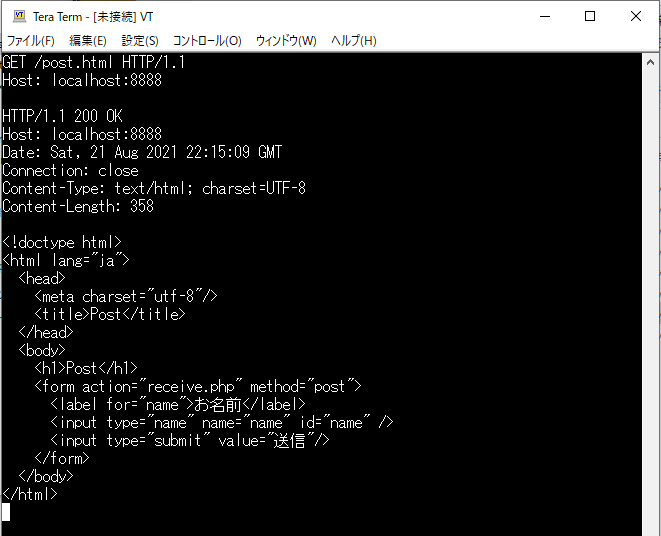
\includegraphics[width=11cm]{../img/32-response.png}
\vspace{3mm}

\newsavebox{\htmltext}
\setbox\htmltext=\vbox{\hsize 13cm
\begin{verbatim}
 HTTP/1.1 200 OK
 Host: localhost:8888
 Date: Sat, 21 Aug 2021 22:15:09 GMT
 Connection: close
 Content-Type: text/html; charset=UTF-8
 Content-Length: 358

 <!doctype html>
 <html lang="ja">
   <head>
     <meta charset="utf-8">
     <title>Post</title>
   </head>
   <body>
     <h1>Post</h1>
     <form action="receive.php" method="post">
       <label for="name">お名前</label>
       <input type="text" name="name" id="name" >
       <input type="submit" value="送信">
     </form>
   </body>
 </html>
\end{verbatim}
}

\fbox{\usebox{\htmltext}}

ブラウザの画面には以下のようにレンダリングされる。

\vspace{3mm}
\begin{tabular}{c|} \hline
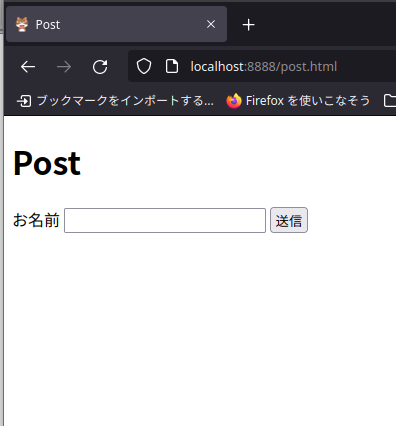
\includegraphics[width=8cm]{../img/31-post.png} \\ \hline
\end{tabular}
\vspace{3mm}


ここでユーザーは名前を入力し、送信ボタンを押して、Webサーバーに
入力した情報を送信する。

このとき、post.html には、以下のように送り先が指定されている。

\vspace{3mm}
\begin{tcolorbox}
$<$form action=''receive.php'' method=''post''$>$
\end{tcolorbox}
\vspace{3mm}

これは、送り先が ``receive.php'' で、送信方法が ``post''送信であるという指定である。

まず、Webサーバーに、クライアント(ブラウザ)から送信された情報を受け取るための
ファイル ''receive.php'' を作成する。``test''フォルダに以下の内容で作成する。

\begin{lstlisting}[caption=receive.php]
<?php
 $name = $_POST['name'];
?>
 <!doctype html>
 <html lang="ja">
   <head>
     <meta charset="utf-8"/>
     <title>receive</title>
   </head>
   <body>
     <h1>receive</h1>
     <p>name="<?php echo $name; ?>"</p>
   </body>
 </html>
\end{lstlisting}

これは、クライアントから送られてきた ``name'' の内容を \$name という変数にセットし、
それをブラウザで表示するというものである。

実際に試してみる。
``test''フォルダでコマンドプロンプトを起動し、\fbox{ $>$ php -S localhost:8888 }
として、Webサーバーを起動する。

ブラウザで \fbox{ http://localhost:8888/post.html } にアクセスして、名前を入力して
送信する。

\vspace{3mm}
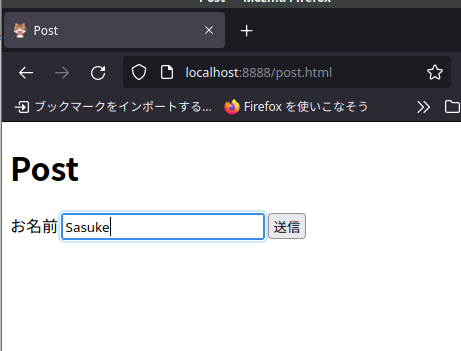
\includegraphics[width=8cm]{../img/33-post-2.png}
\vspace{3mm}

名前を入力して送信すると\dots \dots

\vspace{3mm}
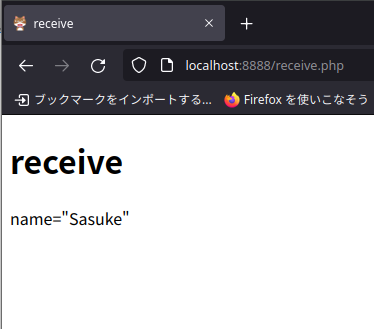
\includegraphics[width=8cm]{../img/34-receive.png}
\vspace{3mm}

このようにブラウザの画面で表示される。

これを TeraTerm を使って Telnet画面でやってみる。
そのことで、ブラウザとWebサーバーでは実際にどういうやりとりが行われているかを確認する。


\subsection{TelnetでのPOST送信のしかた}

``test'' フォルダで Webサーバーが動作している状態で、TeraTerm を起動し、POST送信を
おこなうが、今度は送信文字列が長いので、TeraPad などのエディタで、送信文字列を
あらかじめ作成して、それをコピーして TeraTerm の画面に貼り付けることにする。

\begin{lstlisting}[caption=post-request.txt]
 POST /receive.php HTTP/1.1
 Host: localhost:8888
 Content-Type: application/x-www-form-urlencoded
 Content-Length: 11

 name=Sasuke
\end{lstlisting}

\rightline{(以上をメモ帳などのエディタで書いて、\textsf{post-request.txt}という名前で保存しておく。)}


\begin{enumerate}
 \item 今回は POST送信なので ``POST'' と指定する。\\
       また、送り先として ``receive.php'' を指定する。
 \item これは GET の場合と同じである。
 \item ここでは、ボディ部の長さを伝えている。``name=Sasuke'' で 11バイトである。
 \item 送るデータは urlエンコードされた form の文字列である。
 \item 空行がヘッダ部とボディ部の区切りである。
 \item ``name'' という変数(コントロール名)に ``Sasuke'' という値(文字列)をセットしている。
\end{enumerate}

\hspace{5cm}
\begin{tabular}{|p{10cm}|} \hline
 urlエンコード --- インターネットで漢字など使用できない文字を送る際に使われる文字の変換方式
 。たとえば''山''だと \textsf{\%E5\%B1\%B1} となる。 \\ \hline
\end{tabular}
\vspace{3mm}

6行目の ``name=Sasuke'' は、post.html の以下の部分の記述に相当する。

\begin{tcolorbox}
 $<$input type="text" name=\underline{"name"} id="name" $>$
\end{tcolorbox}

つまり、ユーザーが入力してくれた 値(文字列) に \underline{``name''} という名前をつけて
Webサーバーに送るという意味である。

ここでは、``name'' という文字列がたくさん出てきてややこしいが、たとえば、以下のように
なっていると\dots \dots

\begin{tcolorbox}
 $<$input type="text" name=\underline{"\textsf{namae}"} id="name" $>$
\end{tcolorbox}

post-request.txt の 5行目は、以下のようになる。

\begin{tcolorbox}
 \textsf{namae}=Sasuke
\end{tcolorbox}

要するに、Webサーバーから送られてきた post.html を画面に表示し、ユーザーが
名前を入力し、送信ボタンが押されたとき、

\newsavebox{\posttext}
\setbox\posttext=\vbox{\hsize 13cm
\begin{verbatim}
 POST /receive.php HTTP/1.1
 Host: localhost:8888
 Content-Type: application/x-www-form-urlencoded
 Content-Length: 11

 name=Sasuke
\end{verbatim}
}
\fbox{\usebox{\posttext}}

このようなコマンド文字列が Webサーバーに送られているのである。

そして、POST送信の特徴は、送信されるデータが ボディ部 に埋め込まれるということである。
ということは、SSL通信では暗号化されるということになる。(ヘッダ部は暗号化されない)

今回は送るデータは一つだけだが、POST送信では多くのデータを送ることができる。

\vspace{5mm}
POST送信以外に、GET送信でもデータを送ることができる。以下のようなやりかたで送信する。

\begin{tcolorbox}
 GET /receive.php\textsf{?name=Sasuke} HTTP/1.1
\end{tcolorbox}

今回は GET送信でのデータ送信は詳しくは触れない。


\subsection{TeraTermで POST送信をやってみる}

それでは、TeraTermで POST送信をやってみる。
今回は、実際のやりとりを再現するために、``ローカルエコー'' を ``OFF'' にしてみる。

今までは、TeraTerm の画面では、我々の入力した文字列と、サーバーが送り返してきた文字列を
両方とも表示していた。
しかし実際は、我々が入力した文字列はサーバーに送られてしまい、我々は見ることはできない
はずである。
それでは仕事がやりにくいので、telnetプログラムには、ユーザーが入力した文字列をサーバーに
送ると同時に、ユーザーにも表示してくれる機能がついている。
それが ``ローカルエコー'' で、それを ``ON'' にすることで実現できる。

今までは TeraTerm の画面に直接文字列を入力していたので、''ローカルエコー'' が ''ON'' の
ほうがやりやすかった。
今回は、エディタで文字列を準備しておいて、TeraTermの画面には貼り付けるだけなので、
``ローカルエコー'' を ``OFF'' にしてもできる。

``ローカルエコー'' を ``OFF'' にするには、2つの方法がある。
\begin{enumerate}
 \item 設定ファイル(TERATERM.INI) を書き変える。
 \item 一時的に変更する。
\end{enumerate}

今回は、``一時的に変更する'' のほうでやってみる。

手順をまとめると以下になる。

\vspace{3mm}

\newsavebox{\itemtext}
\setbox\itemtext=\vbox{\hsize 15cm
\begin{enumerate}
 \item TeraTermを起動する。
 \item ``設定'' --- ``端末'' を選択して ``端末の設定''画面で、``ローカルエコー''のチェックをはずす。
 \item ``post-request.txt'' の内容をコピーする。
 \item ``編集'' --- ``貼り付け'' を選択。
 \item 貼り付ける文字列の確認画面が開くので、それをOKする。
 \item 黒い画面になるので、``$<$Enter$>$''キーを押す。
 \item サーバーから文字列が送られてくる。
\end{enumerate} 
}

\fbox{\usebox{\itemtext}}

以下、ひとつひとつの手順を確認する。


\newpage
\textsf{1.} TeraTermを起動する。

\vspace{3mm}
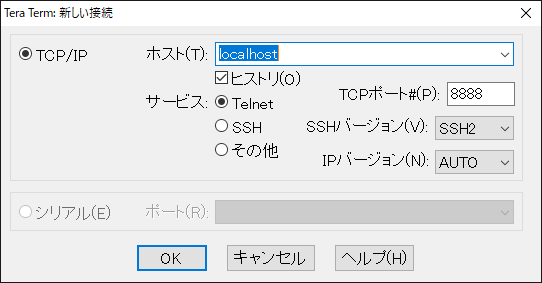
\includegraphics[width=10cm]{../img/41-post-connect.png}
\vspace{3mm}

\textsf{2.} ``設定'' --- ``端末'' を選択して ``端末の設定''画面で、``ローカルエコー''のチェックをはずす。

\vspace{3mm}
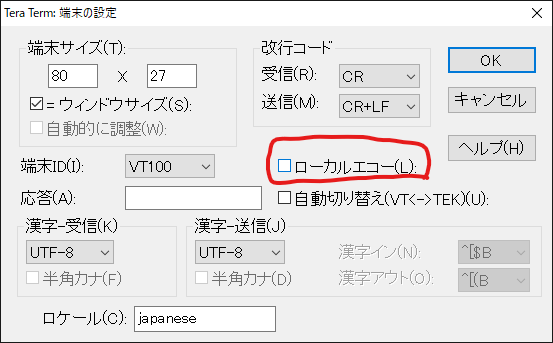
\includegraphics[width=10cm]{../img/42-localecho-off.png}
\vspace{3mm}

\textsf{3.} ``post-request.txt'' の内容をコピーする。

\vspace{3mm}
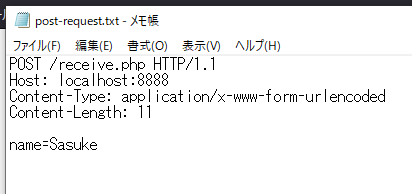
\includegraphics[width=10cm]{../img/43-post-copy.png}
\vspace{3mm}

余分な''空行''などコピーしないように ``Sasuke'' までをコピーする。

\newpage
\textsf{4.} TeraTermの黒い画面で ``編集'' --- ``貼り付け''

\vspace{3mm}
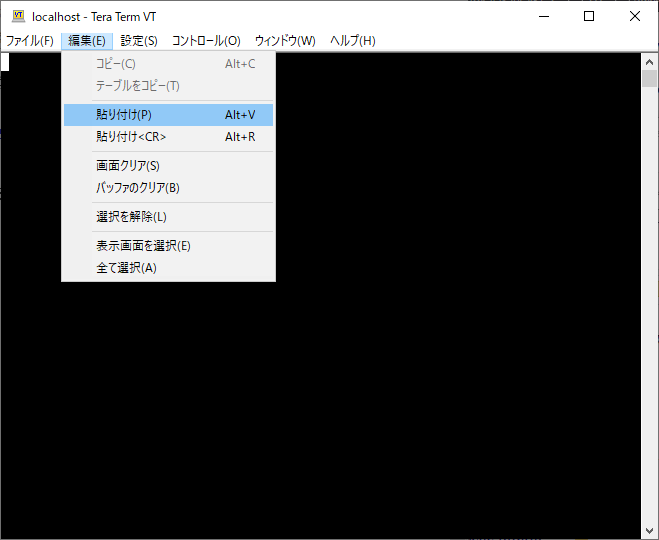
\includegraphics[width=10cm]{../img/44-edit-paste.png}
\vspace{3mm}

\textsf{5.} 貼り付ける文字列の確認画面が開くので、それをOKする。

\vspace{3mm}
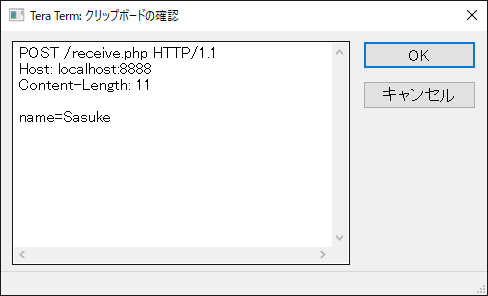
\includegraphics[width=10cm]{../img/45-paste-confirm.png}
\vspace{3mm}

\newpage
\textsf{6.} 黒い画面になるので、``$<$Enter$>$''キーを押す。

こちらから貼り付けた文字列はサーバーへ送られたので、画面には出ていない。
これが ``ローカルエコー・オフ'' ということである。

\vspace{3mm}
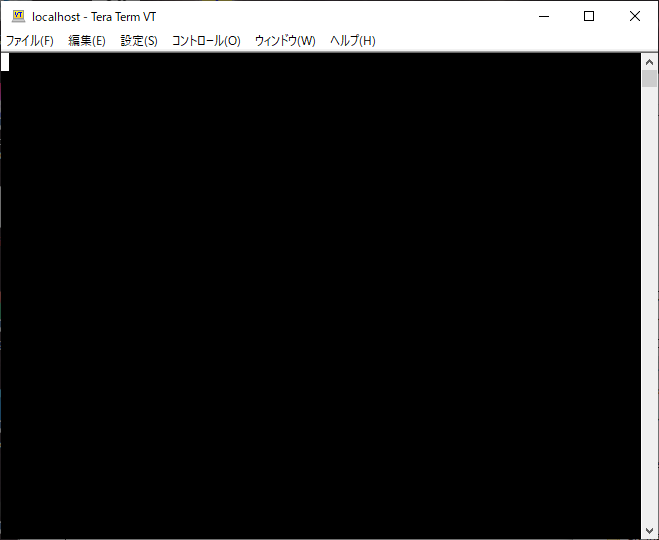
\includegraphics[width=10cm]{../img/46-black.png}
\vspace{3mm}

\textsf{7.} サーバーから文字列が送られてくる。

\vspace{3mm}
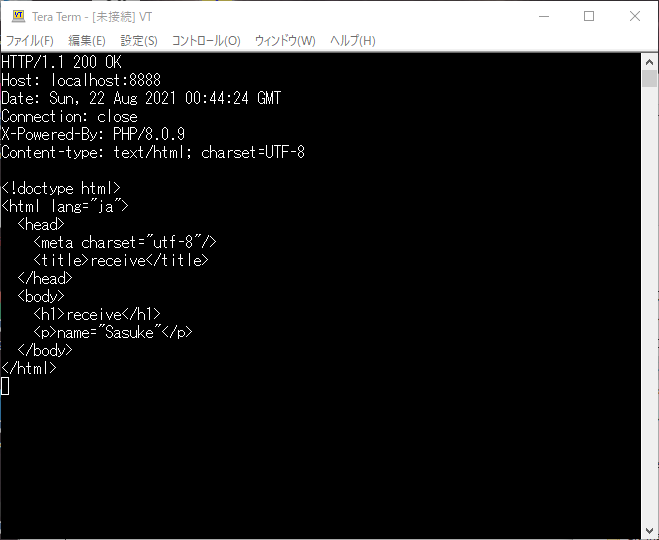
\includegraphics[width=10cm]{../img/47-post-result.png}
\vspace{3mm}

送られてきた文字列は、以下である。

\newsavebox{\htmlbox}
\setbox\htmlbox=\vbox{\hsize 13cm
\begin{verbatim}
HTTP/1.1 200 OK
Host: localhost:8888
Date: Sun, 22 Aug 2021 03:15:13 GMT
Connection: close
X-Powered-By: PHP/8.0.9
Content-type: text/html; charset=UTF-8

<!doctype html>
<html lang="ja">
  <head>
    <meta charset="utf-8"/>
    <title>receive</title>
  </head>
  <body>
    <h1>receive</h1>
    <p>name="Sasuke"</p>
  </body>
</html>
\end{verbatim}
}
\fbox{\usebox{\htmlbox}}

ヘッダ部は GET送信のときとそんなに変りはない。
5行目で PHP で処理したことが明記されている。

ボディ部のほうは、``receive.php''の内容であるが、\verb!<?php ... ?>! で記述された
部分はない。

特に、\verb!<?php echo $name; ?>! で記述された部分は 文字列''Sasuke''
に置き変わっている。









\end{document}

%% 修正時刻: Sat May  2 15:10:04 2020



%% 修正時刻: Thu Aug 26 08:47:59 2021
